
%% %-----Preámbulo ----- % % %

%Tipo de Documento: 
\documentclass{article} 

%Este paquete es utilizado para personalizar elementos por idioma: 
\usepackage[spanish ,mexico]{babel} 
  
%Este paquete es utilizado para la codificación de entrada: 
\usepackage[utf8]{inputenc} 

%Este paquete se utiliza para separar el texto en columnas
\usepackage{multicol}
\setlength{\columnseprule}{1pt}

%Paquete para fórmulas matemáticas
\usepackage{amssymb}

%Paquete para cargar gráficos
\usepackage{graphicx}

%Paquete para escribir tipo máquina de escribir
\usepackage{verbatim}

%Paquete para poner índice
\usepackage{makeidx}

%Otras declaraciones: 
\title{Mini -Tutorial de los elementos de \LaTeX} 
\author{Sof\'ia Marina Figueroa Due\~nas} 
\date{13 de julio de 2018}
    
%%%----Cuerpo----- %%%
\makeindex
\begin{document}  
\maketitle 
\newpage
\tableofcontents
\newpage
\section{Caracteres especiales}
\label{sec:car_es}
Para introducir caracteres especiales (o comandos) se utiliza generalmente la diagonal invertida ``\textbackslash'' antes del s\'imbolo deseado.

Dos backslashes seguidos (\textbackslash \textbackslash) son interpretados como un retorno de carro. \\Si lo que quiero es escribir:\\
\begin{tabular}{c c}
Llave de apertura 	& \{	\\
Llave de cierre		& \}	\\
Porcentaje			& \%	\\
Pesos				& \$	\\
Ampersant			& \&	\\
Gatito				& \#	\\
Gorrito				& \^\	\\
Tilde ondulada		& \~\	\\
Diagonal invertida	& \textbackslash	\\
\end{tabular}


\section{Referencias Cruzadas}
Los comandos utilizados para usar referencias cruzadas a figuras, tablas y segmentos 
contenido en el documento son:


\begin{center}
\textbackslash label{marcador}\\
\textbackslash ref{marcador}\\
\textbackslash pageref{marcador}
\end{center}



donde ``marcador'' es un identificador elegido por el usuario. En el texto final del comando
``\textbackslash ref'' aparecer\'a como el n\'umero de secci\'on, subsecci\'on, figura, tabla o teorema
que representa su comando ``\textbackslash label'' correspondiente; mientras el comando
``\textbackslash pageref'' aparecer\'a como el n\'umero de p\'agina en el que se encuentra su comando
``\textbackslash label'' correspondiente.\\

En el iguiente ejemplo se le a\~nadi\'o a la secci\'on de Caracteres Especiales el comando:``\textbackslash label(marcador)'', al final de la l\'inea se le a\~nadi\'o la referencia con ``\textbackslash ref(marcador)'':

Tenemos referencia la secci\'on anterior sobre caracteres especiales enseguida \ref{sec:car_es}

Sin embargo por la cantidad de palabras utilizada se ve poco est\'etica la referencia por lo que se le antepone el caracter `` \~\ '' al comando ``\textbackslash ref(marcador)'' y \LaTeX acomodar\'a las palabras para que se vea un poco mejor como a continuaci\'on:

Tenemos referencia de la secci\'on anterior sobre los caracteres especiales enseguida \ref{sec:car_es}

Ahora en ocasiones no s\'olo se quiere hacer referencia a el n\'umero de secci\'on (subsecci\'on etc) sino a su ubicaci\'on en el documento. Es decir su p\'agina. Para esto se utiliza el comando ``\textbackslash pageref''

Tenemos la referencia de la p\'agina a la secci\'on anterior sobre caracteres especiales seguida \pageref{sec:car_es}


\section{Notas al pie}
Colocar notas al pie es bastante sencillo
\footnote{Para quien sabe c\'omo hacerlo, o bien tiene Internet en su compu}.
Simplemente se utiliza el comando:\\

\textbackslash footnote\{Texto\}\\

deber\'an ser ubicadas siempre luego de la palabra que se refieren y su numeraci\'on se maneja autom\'aticamente.


\section{Listas}
Crear listas es muy sencillo. Existen dos tipos de listas, numeradas y no numeradas. A continuaci\'on se muestran los dos tipos.

\subsection{Listas numeradas}
El comando a utilizar (enumarate) se ingresa dentro de un ambiente \textbackslash begin \{enumerate\} y se finaliza con un \textbackslash end y se debe escribir un \textbackslash item para cada inciso:

\begin{multicols}{2} 
\noindent
\textbackslash begin\{enumerate\}\\	
\textbackslash item inciso 1\\
\textbackslash item inciso 2\\
\textbackslash end \{enumerate\}
\columnbreak
\begin{enumerate}
\item inciso 1\\
\item inciso 2
\end{enumerate}
\end{multicols}

Otro ejemplo de una lista numerada:

\begin{multicols}{2}
\noindent
\textbackslash begin\{numerate\}\\
\textbackslash item Este es el primer elemento\\
\textbackslash item Este es el segundo\\
elemento\\
\textbackslash item Este es el tercer elemento\\
\textbackslash end\{enumerate\}
\columnbreak
\begin{enumerate}
\item Este es el primer elemento
\item Este es el segundo elemento
\item Este es el tercer elemento
\end{enumerate}
\end{multicols}


\subsection{Listas no numeradas}
De igual forma se ingresa en un ambiente el comando, en este caso (itemize), para obtener una lista no numerada:

\begin{multicols}{2} 
\noindent
\textbackslash begin\{itemize\}\\	
\textbackslash item inciso 1\\
\textbackslash item inciso 2\\
\textbackslash end \{itemize\}
\columnbreak
\begin{itemize}
\item inciso 1
\item inciso 2
\end{itemize}
\end{multicols}

Otro ejemplo de lista no numerada:

\begin{multicols}{2} 
\noindent
\textbackslash begin\{itemize\}\\	
\textbackslash item Estes es el primer elemento\\
\textbackslash item Este es el segundo elemento\\
\textbackslash item Este es el tercer elemento
\textbackslash end \{itemize\}
\columnbreak
\begin{itemize}
\item Este es el primer elemento
\item Este es el segundo elemento
\item Este es el tercer elemento
\end{itemize}
\end{multicols}

\subsubsection{Listas Personalizadas}
Se puede poner un marcador personalizado para las listas no numeradas o itemize, simplemente usando la misma sintaxis anterior, pero a\~nadiendo entre [ ] el marcador a utilizar\\
Como por ejemplo:\\

\begin{multicols}{2} 
\noindent
\textbackslash begin\{itemize\}\\	
\textbackslash item [pri]Este es el primer\\
elemento\\
\textbackslash item [seg]Este es el segundo\\ 
elemento\\
\textbackslash item [ter]Este es el tercer\\ 
elemento\\
\textbackslash end \{itemize\}
\columnbreak
\begin{itemize}
\item[pri]Este es el primer elemento
\item[seg]Este es el segundo elemento
\item[ter]Este es el tercer elemento
\end{itemize}
\end{multicols}

\newpage
\subsubsection{Anidaciones}
Se pueden anidar listas de otras listas sin importar el tipo, y se puede hacer tantas veces como se necesite:

\begin{multicols}{2}
\noindent
\textbackslash begin \{itemize\}\\
\textbackslash item Este es el primer\\
elemento\\
\hspace*{1cm}\textbackslash begin\{enumerate\}\\
\hspace*{1cm}\textbackslash item Este es el primer\\
\hspace*{1cm}elemento\\
\hspace*{1cm} \textbackslash Este es el primer\\\hspace*{1cm}elemento\\
\hspace*{1cm} \textbackslash end\{enumerate\}\\
\textbackslash item Este es el segundo\\
elemento\\
\hspace*{1cm} \textbackslash begin\{enumerate\}\\
\hspace*{1cm} \textbackslash Este es el primer\\\hspace*{1cm}elemento\\
\hspace*{1cm} \textbackslash Este es el primer\\\hspace*{1cm}elemento\\
\hspace*{1cm} \textbackslash end\{enumerate\}\\
\textbackslash end\{itemize\}
\columnbreak
\begin{itemize}
\item Este es el primer elemento
	\begin{enumerate}
	\item Este es el primer elemento
	\item Este es el primer elemento
	\end{enumerate}
\item Este es el segundo elemento
	\begin{enumerate}
	\item Este es el primer elemento
	\item Este es el primer elemento
	\end{enumerate}
\end{itemize}
\end{multicols}


\section{Tablas}
El ambiente ``tabular'' puede ser utilizado para crear tablas con l\'ineas verticales y
horizontales opcionales. \LaTeX\ determina el ancho de las columnas autom\'aticamente.
El par\'ametro ``formato'' del comando:


\begin{center}
\textbackslash begin\{tabular\}\{formato\}\\
Texto\\
\textbackslash end\{tabular\}
\end{center}


define el formato de la tabla. Se puede usar los siguientes par\'ametros:

\begin{itemize}
\item ``l'' Columna con texto alineado a la izquierda.
\item ``r'' Columna con texto alineado a la derecha.
\item ``c'' Columna con texto centrado.
\item ``p\{ancho\}'' Columna con texto justificado y saltos de l\'inea.
\item ``|'' L\'inea vertical.
\end{itemize} 


En el ambiente ``tabular'':
\begin{itemize}
\item ``\&'' Salta a la siguiente columna.
\item ``\textbackslash \textbackslash'' Comienza con una nueva l\'inea
\item ``\textbackslash hline'' Inserta una l\'inea horizontal.
\item ``\textbackslash cline\{j-i\}'' Agrega una l\'inea parcial, donde ``j'' e ``i'' son
los n\'umeros de columna en los cuales la nueva l\'inea se debe extender.
\item Separaciones verticales:
\begin{itemize}
\item \textbackslash smallskip salto peque\~no
\item \textbackslash medskip salto mediano
\item \textbackslash bigskip salto grande
\end{itemize}
\end{itemize}

Realizar tablas es bastante sencillo. A continuaci\'on he creado ya una tabla en menos de 1 minuto.

\bigskip
\begin{multicols}{2}
\noindent
\textbackslash begin\{tabular\}\{\textbar \hspace*{1mm}c\hspace{1mm}\textbar\hspace{1mm}c\hspace*{1mm} \textbar\}\\
\textbackslash hline\\
orden \& n\'umero\\
\textbackslash hline\\
\\
1\quad \& 2\textbackslash \textbackslash \\
2\quad \& 3\textbackslash \textbackslash \\
3\quad \& 5\textbackslash \textbackslash \\
4\quad \& 7\textbackslash \textbackslash \\
5\quad \& 11\textbackslash \textbackslash \\
\textbackslash hline\\
\textbackslash end\{tabular\}\\
\columnbreak
\begin{tabular}{|c | c|}
\hline
orden & n\'umero\\
\hline
1	&2\\
2	&3\\
3	&5\\
4	&7\\
5	&11\\
\hline 
\end{tabular}
\end{multicols}

Otro ejemplo:

\begin{multicols}{2}
\noindent
\textbackslash begin\{tabular\}\{\textbar \hspace*{1mm}r\hspace{1mm}\textbar\hspace{1mm}l\hspace*{1mm} \textbar\}\\
\textbackslash hline\\
7C0 \& hexadecimal \textbackslash \textbackslash \\
3700 \& Octal \textbackslash \textbackslash \quad \textbackslash cline\{2-2\}\\
11111000000 \& binario \textbackslash \textbackslash \\
\textbackslash hline \textbackslash hline\\
1984 \& decimal \textbackslash \textbackslash \\
\textbackslash hline\\
\textbackslash end\{tabular\}\\

\columnbreak

\begin{tabular}{| r | l |}
\hline
7C0	& Hexadecimal \\
3700 & Octal \\ \cline{2-2}
11111000000 & binario \\
\hline	\hline
1984 & decimal \\
\hline
\end{tabular}
\end{multicols}


\section{F\'ormulas matem\'aticas}

Para utilizar f\'ormulas matem\'aticas se pueden emplear diversos ambientes.

\subsection{F\'ormulas en l\'inea}
Para escribir dentro de una misma l\'inea (inline) se muestran mezcladas en el texto.
Para f\'ormulas cortas, tambi\'en podemos usar \textbackslash \$ de manera similar a \textbackslash [.

Ejemplo:

Def\'inase la siguiente funci\'on
$f:(0,\infty)\to\mathbb{R}$
como:
\[
f(x)=\frac{\ln x}{x^2}
\]
entonces:
$$\lim_{x\to\infty}f(x)=0$$

Otra forma de obtener este tipo de f\'ormulas es con el ambiente math.

\begin{center}
\begin{math}
f(x)=\frac{\ln x}{x^2}
\end{math}
\end{center}

\subsection{F\'ormulas independientes}
Si nuestra intenci\'on es mostrar una f\'ormula independiente del texto,
entonces usaremos un entorno displaymath que se puede abreviar con
``\textbackslash [f(x) \textbackslash]''. Mediante el ejemplo:
\begin{displaymath}
\sum_{i=0}^{n}\frac{1}{i!}x 
\end{displaymath}

\subsection{F\'ormulas de varias l\'ineas}
Los entornos equation y displaymath crean f\'ormulas de una sola l\'inea. Para obtener una serie de ecuaciones en distintas l\'ineas, usaremos el 
entorno ``eqnarray'' y una sintaxis parecida a las tablas: 
\begin{eqnarray} 
y = (x-2)^2+(x-4)^2 
\nonumber \\ 
y = (x^2-4x+4)+(x^2-8x+16) \\ 
y = 2x^2-12x+20 
\end{eqnarray}


\section{Justificaci\'on de p\'arrafos} 
\subsection{Texto centrado} 

\subsubsection{Centrar una l\'inea} 
Para centrar una l\'inea de texto se utiliza el comando \textbackslash centerline\{Texto\}\\ \centerline{Ejemplo de una linea centrada} 

\subsubsection{Centrar varias l\'ineas y otros materiales \LaTeX} 
Para centrar texto que se extienda por m\'as de una l\'inea y otro tipo de materiales , se
utiliza el entorno:\\ 
\textbackslash begin\{center\} ... (Texto)... \textbackslash end\{center\}.\\
\LaTeX\ a\~nade espacio vertical antes y despu\'es del material centrado. 

\begin{center} 
Este es un ejemplo de como centrar en \LaTeX\ cualquiera de los materiales producidos. 
\end{center}


\section{Formato de fuente}

\subsection{Tipos de fuentes \LaTeX}
Las fuentes que usa \LaTeX\ son las llamadas fuentes CM (Computer MModern Fonts), que fueron
dise\~nadas por Donald Knuth. Para acceder a cualquier tipo de fuente se utiliza la sintaxis: 
\textbackslash (Comando fuente)\{Texto en la fuente\}

Ejmplo:

\begin{tabular}{l  r}

\textrm{romana normal} & \textbackslash textrm\{texto\}\\
\textsf{sans serif} & \textbackslash textsf\{texto\}\\
\texttt{mono-espaciada (typewriter)} & \textbackslash texttt\{texto\}\\
\textit{Cursiva o italica} & \textbackslash textit\{texto\}\\
\textbf{negrilla} & \textbackslash textbf\{texto\}\\
\textsl{Inclinada (slanted)} & \textbackslash textsl\{texto\}\\
\textsc{Versalitas (small caps)} & \textbackslash textsc\{texto\}\\
\end{tabular}


\subsection{Combinaci\'on de fuentes}
Los comandos para utilizar las fuentes se pueden combinar para obtener fuentes con caracter\'isticas combinadas.

\textsc{\'Esta es una \textit{frase escrita}} \textsl{combinando \textbf{varios \textsf{tipos de 
fuentes}}} propias \textrm{de} \LaTeX.


\subsection{Modos enf\'aticos} 
Cada uno de los tipos de fuentes b\'asico tiene su modo enf\'atico, el cual se obtiene por medio 
del comando: \\
\centerline{\textbackslash emph\{texto\}} 

Ejemplos: 

Modo enf\'atico, 
\emph{Modo enf\'atico}.\\ 
\textit{Modo enf\'atico, 
\emph{Modo enf\'atico}.}\\ 
\texttt{Modo enf\'atico, 
\emph{Modo enf\'atico}.}\\ 
\textsc{Modo enf\'atico, 
\emph{Modo enf\'atico}.}\\


\subsection{Tama\~no de fuente} 
El tama\~no de la letra por defecto es 10pt, pero en las opciones del comando 
\textbackslash documentclass se pueden establecer los tama\~nos 11pt y 12pt. 
Adicionalmente se puede cambiar el tama\~no para partes particulares de un 
documento, los cuales son relativos a la fuente escogida para el documento. 

\begin{itemize} 
\item{\tiny tiny} 
\item{\scriptsize scriptsize} 
\item{\footnotesize footnotesize} 
\item{\small small} 
\item{\normalsize normalsize} 
\item{\large large} 
\item{\Large Large} 
\item{\LARGE LARGE} 
\item{\huge huge} 
\item{\Huge Huge} 
\end{itemize} 


\subsubsection{Uso de los tama\~nos y combinaci\'on con tipos de fuentes} 
Para hacer uso de los tama\~nos relativos de las fuentes, estos se pueden declarar en cualquier parte del documento; si se desea que su alcance este limitado, es necesario que este dentro de una declaraci\'on global o un entorno.\\ 
{\small \LaTeX\ \textsc{tiene predefinidos {\tiny 10 tamanos} de fuentes \textit{\Large 
relativos a la fuente} actual del \textbf{\normalsize documento}.}} 

\subsection{Texto subrayado}
Para subrayar cualquier texto de un documento \LaTeX\
se utiliza el comando \textbackslash underline\{texto\}.

\underline{Este es un ejemplo de texto subrayado}


\section{Cajas}
\parbox{0.3\textwidth}{Una caja es un elemento que \LaTeX\ trata como si fuera una sola letra:}

\parbox{0.7\textwidth}{noimporta cuan grande es, \LaTeX\ nunca la divide en partes. Existen varios tipos de cajas que se pueden crear;}

\parbox{\textwidth}{con borde sin borde, con una sola l\'inea o con varias, un ancho predefinido, con una justificaci\'on adem\'as de que se puede insertar material distinto a un texto, como gr\a'ficos.}

\medskip
El texto anterior que se incluy\'o dentro de cajas mediante el comando
\textbackslash parbox\{Tama\~no\}\{Texto\}

\subsection{Cajas con una sola l\'inea de texto} 
\begin{itemize}
\item \textbackslash mbox\{texto\} crea una caja con bordes invisibles que contiene al texto. 
\item \mbox{caja con bordes invisibles que contiene al texto} 
\item \textbackslash fbox\{texto\} crea una caja con bordes visibles que contiene al texto. 
\item \fbox{caja con bordes visibles que contiene al texto}
\end{itemize}

\section{Inclusi\'on de archivos} 
\subsection{Gr\'aficos} 
Los formatos m\'as recomendables para su uso son el Encapsulated PostScript ( EPS) y el formato PostScript (PS). Si usamos PDF \LaTeX\, los formatos m\'as comunes son PDF, PNG, JPG o GIF. Los archivos son insertados dentro del fichero \LaTeX\ mediante el comando \textbackslash includegraphics[formato]\{imagen\} 
como por ejemplo:

\begin{figure}[h]
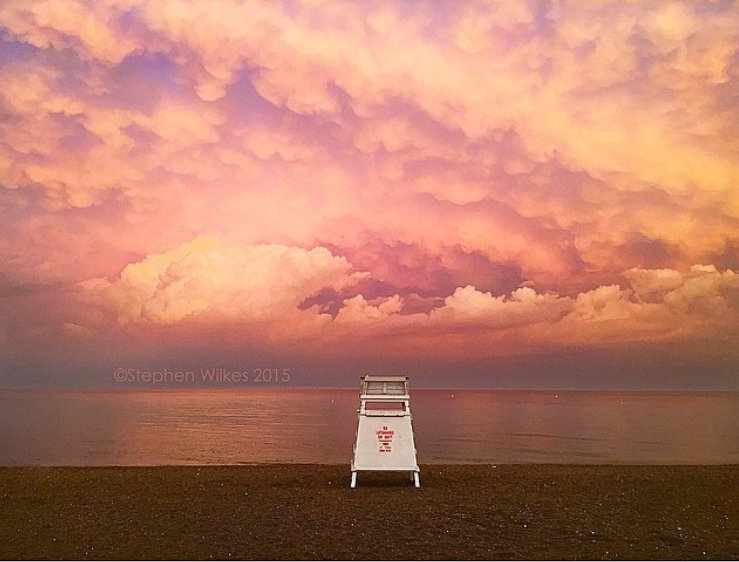
\includegraphics[scale=.16]{lago}
\centering
\caption{\'Esta es una im\'agen de ejemplo para revisar la forma en que se alinean los gr\'aficos y el texto.}
\end{figure}


Tambi\'en podemos obtener un mejor acomodo de las im\'agenes con el texto circundante para un prop\'osito est\'etico insert\'andolas en el ambiente figure, como por ejemplo: \\
\newpage
Las opciones disponibles para \textbackslash includegraphics son:

\begin{tabular}{l l}
\hline 
\hline 
width & Anchura del gr\'afico (escal\'andolo si es necesario).\\ 
height & Altura del gr\'afico (escal\'andolo si es necesario).\\ 
scale & Define un factor de escala a aplicar en ambas direcciones.\\
angle & Especifica un \'angulo de rotac\'oin en grados\\ 
&(en sentido positivo).\\ 
clip & Es un par\'ametro l\'ogico. Si se le asigna el valor true el\\ 
&gr\'afico sera recortado (no escalado) a las dimensiones\\ 
&especificadas.\\ 
trim & Un elemento que se lleva bien con clip , debido a que\\ 
& con trim se asignan las dimensiones a recortar.  \\
\hline
\hline
\end{tabular}
\medskip

\begin{figure}[h]
\centering
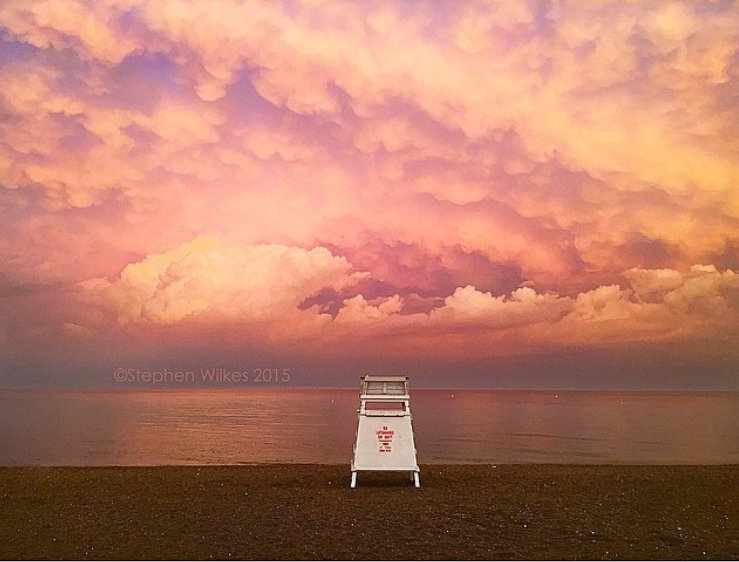
\includegraphics[scale=.16]{lago}
\caption{Este es una im\'agen de ejemplo para revisar la forma en que se acomoda la im\'agen.}
\end{figure}

\begin{figure}[h]
\centering
\begin{tabular}{cc} 
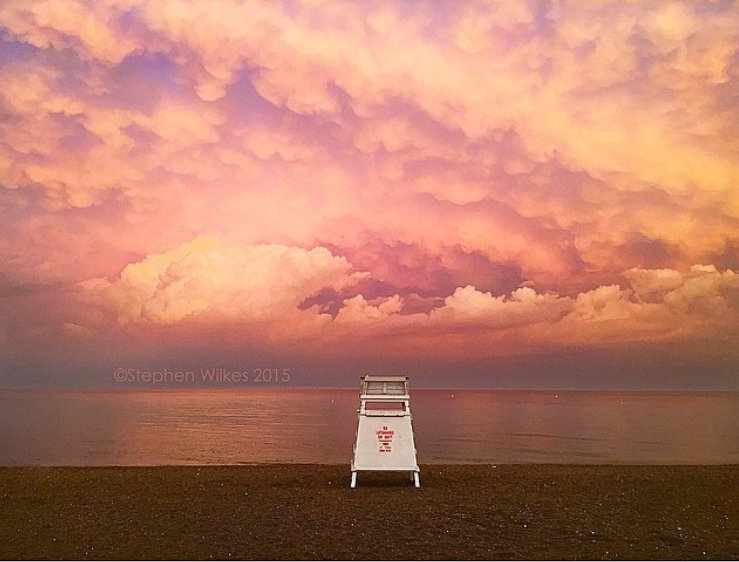
\includegraphics[width= 2 cm, height=6 cm]{lago}& 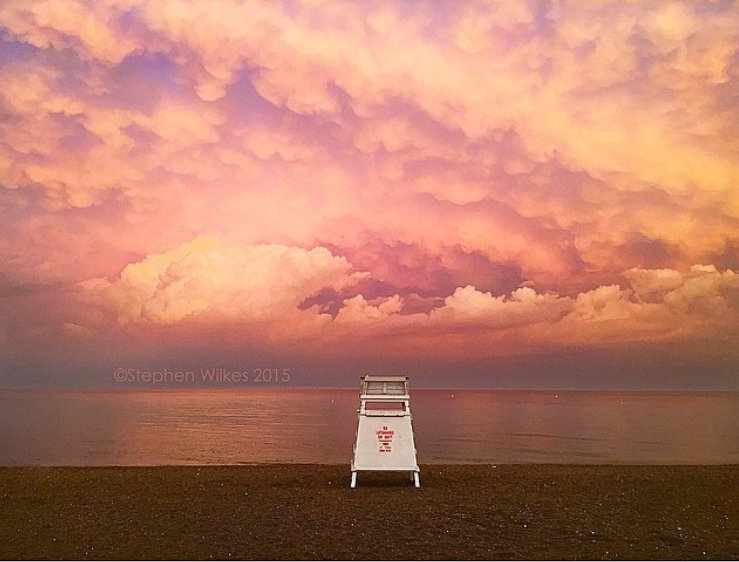
\includegraphics[width= 5 cm, height=3 cm]{lago} 
\end{tabular} 
\caption{Usando width y height} 
\end{figure}

\begin{figure}[h]
\centering
\begin{tabular}{cc} 
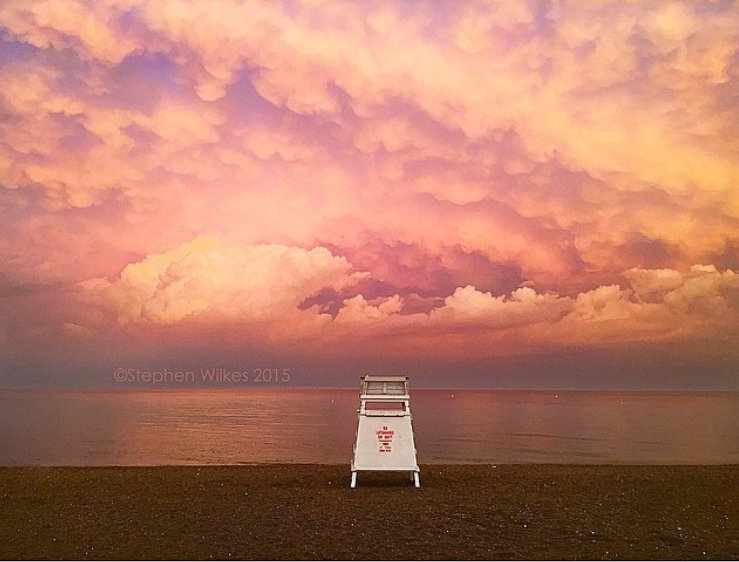
\includegraphics[scale=0.05]{lago}& 
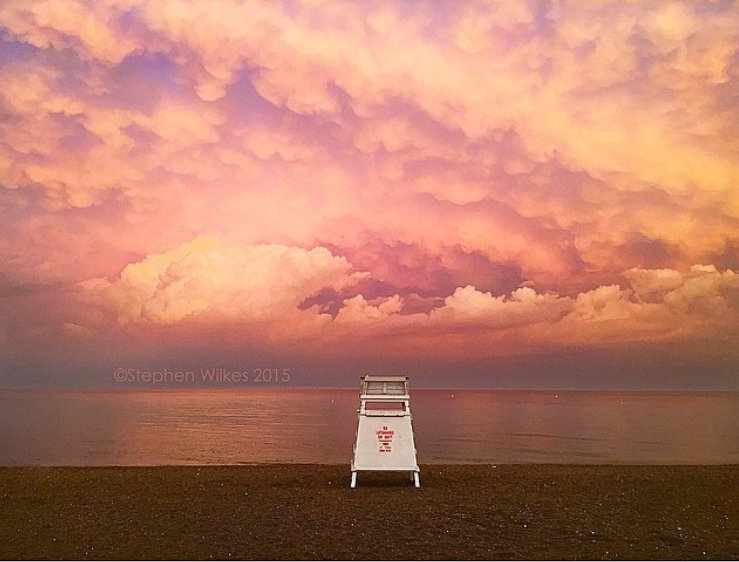
\includegraphics[scale=0.15]{lago} 
\end{tabular} 
\caption{Usando scale} 
\end{figure}

\begin{figure}[h] 
\centering
\begin{tabular}{cc} 
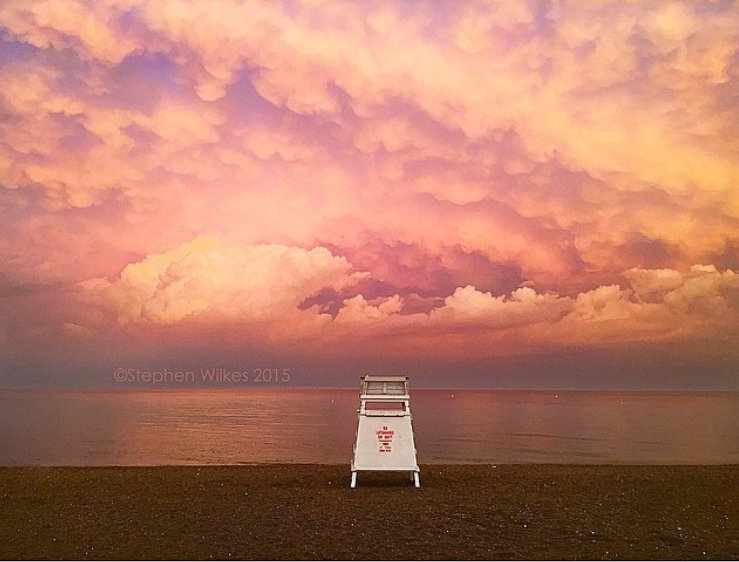
\includegraphics[scale=0.1, angle=40]{lago}& 
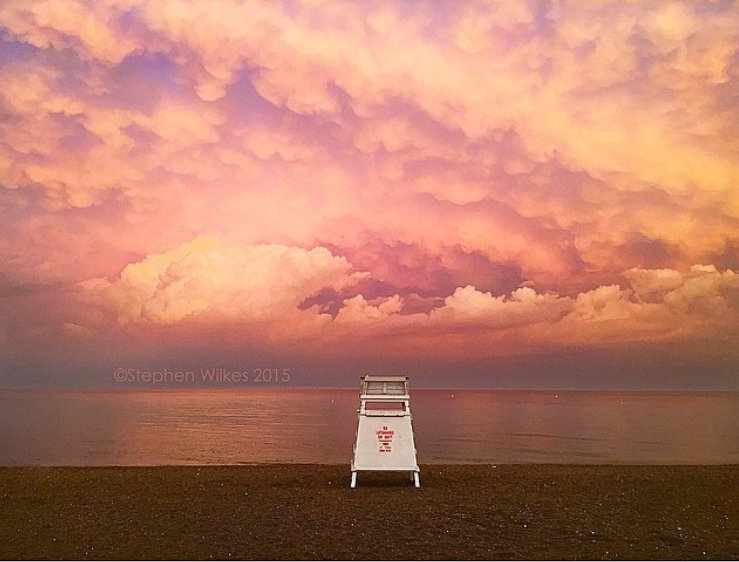
\includegraphics[scale=0.1, angle=20]{lago} 
\end{tabular} 
\caption{Usando angle} 
\end{figure} 

\begin{figure}[!]
\centering
\begin{tabular}{cc} 
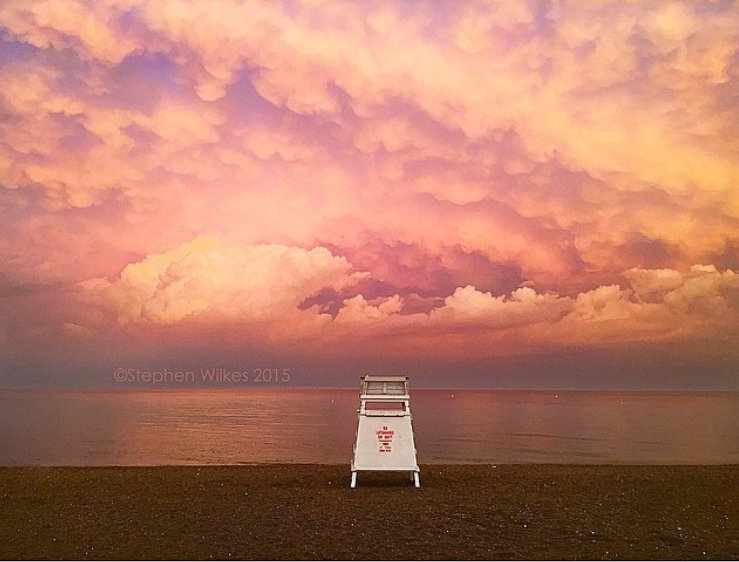
\includegraphics[height=2.5cm, width=4cm, trim={4cm 8cm 4cm 2cm}, clip]{lago}&  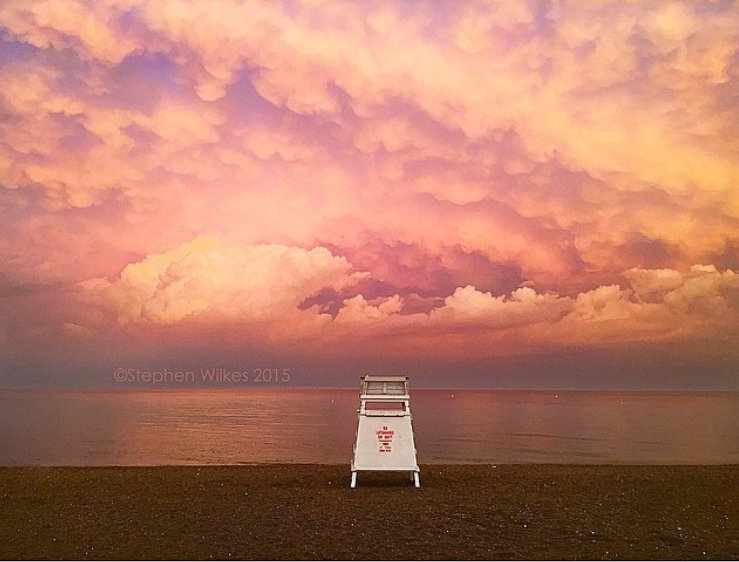
\includegraphics[height=2.5cm, width=4cm]{lago} 
\end{tabular} 
\caption{Usando trim y clip} 
\end{figure}

\subsection{Ubicaci\'on de gr\'aficos}
Por defecto, \LaTeX\ busca los archivos gr\'aficos en los directorios predeterminados por \TeX. Adem\'as , es posible especificar directorios para la busqueda de estos archivos mediante el comando \textbackslash graphicspath. La sintaxis es:\\ 
\textbackslash
graphicspath \{ \{dir1\textbackslash \}\{dir2\textbackslash \}\} 



\section{Comandos personalizados} 
\LaTeX\ nos permite crear nuestros propios comandos para lograrlo usamos el comando:
\textbackslash newcommand\{\textbackslash Nombre\}\{Definicion\}. 
Es bastante \'util cuando en un documento repetimos mucho una palabra dific\'il de escribir o una frase o una ecuaci\'on. 

Un ejemplo de comando personalizado es: 

\newcommand{\UG}{\textit{
Universidad de Guanajuato}, 
Campus Guanajuato, 
Divisi\'on de Ingenier\'ias 
Sede Bel\'en}

Soy estudiante de la \UG. 
Me gusta estudiar en la \UG.


\medskip 
Otro ejemplo es evitarnos escribir \textbackslash textbackslash cuando 
queremos mostrar un comando, por lo tanto lo reduciremos a: 
\textbackslash newcommand\{\textbackslash dinv\}\{\textbackslash textbackslash\} 
\newcommand{\dinv}{\textbackslash}
Ya se puede escribir una ``\dinv'' mas f\'acilmente.

\subsection{Matando dos p\'ajaros de un tiro: Matrices y Comandos...}
Para crear matrices de 3 x 3, como por ejemplo la matriz identidad entre llaves \ref{eq:identidad2}, usamos el ambiente \textbf{array}:

\begin{eqnarray}
\left\{
\begin{array}{ccc}
1&0&0\\
0&1&0\\
0&0&1\\
\end{array}
\right\}
\label{eq:identidad2}
\end{eqnarray}

Tambi\'en podemos crear comandos que nos sirvan como funciones para generar 
matrices, como por ejemplo la siguiente matriz: 
\newcommand{\meq}[2]{
\begin{equation} 
\left[ 
\begin{array}{#1} 
#2
\end{array} 
\right] 
\end{equation} 
}

Y podemos llamar a las ecuaciones d\'andole los par\'ametros que queramos as\'i: 
\meq{cc}{1&0\\0&1} 
Podemos notar en la declaraci\'on de la funci\'on que los s\'imbolos \# dan el espacio para poder llamar a la funci\'on insertando los p\'arametros que necesitemos. 


\section{Ambientes personalizados} 
El siguiente ejemplo cambia el formato del texto, asignando un cierto espacio entre lo que se 
escribe y a\~nade un asterisco al inicio y otro al final. 
\newenvironment{titulito}{*\hspace{\stretch{1}}}{\hspace{\stretch{1}}*}

\medskip 
\begin{titulito}
As\'i se utiliza 
\end{titulito}


\section{Verbatim -Formato C\'odigo} 
El entorno \textbf{verbatim} nos permite escribir un texto como si lo hici\'eramos en una m\'aquina de escribir: hay que indicar donde se partir\'an las l\'ineas mediante retornos de carro, respeta el n\'umero de espacios dejados, permite utilizar directamente los caracteres reservados y utiliza la familia typewriter.\\ 
Estos comandos resultan especialmente \'utiles para escribir salidas o entradas de computadora, comandos o programas a inform\'aticos. En el entorno verbatim no pueden utilizarse argumentos de otros comandos.\\ 
La sintaxis es la siguiente: 
\dinv begin\{verbatim\} ... {texto} ... \dinv end\{verbatim\} 
\medskip 
Ser\'a necesario incluir el paquete \dinv usepackage\{verbatim\}

En el siguiente ejemplo veremos un c\'odigo escrito en lenguaje C. 

\medskip 
\begin{verbatim} 
#include <math.h> 
#include <stdio.h> 
int main() { 
    double a=0.0; 
    double b=5.0; 
    int n=1000; 	
    double dx=(b-a)/(double)n; 
    double sum=0.0; 
    for (double x=a+dx; x<b; x+=dx) 
        sum+=x*x*exp(-x*x); 
	
    sum+=(a*a*exp(-a*a)+b*b*exp(-b*b))/2.0; 
    sum*=dx 

    printf(‘‘Integral= %.2f\n’’, sum); 

    return =0; 
} 
\end{verbatim} 


\section{Referencias bibliogr\'aficas} 
Las referencias bibliogr\'aficas son indispensables para cualquier documento acad\'emico y formal, 
para crear dichas referencias bibliogr\'aficas usamos el ambiente: 
\begin{itemize} 
\item \dinv begin\{thebibliography\}\{numero\} ... \dinv end\{thebibliography \} 
\item Utilizando \dinv bibitem\{name -key\} para la informaci\'on del autor, t\'itulo de referencia,
editorial , a\~no, etc... 
\item El ``name-key'' nos permitir\'a hacer la referencia, en alg\'un lugar del documento, \'unicamente a 
este item. 
\end{itemize} 

\begin{thebibliography}{3} 
\bibitem{asimov} Asimov , I., 
{\it El fin de la eternidad}, 
Ediciones Orbis , S.A., 1977. 

\bibitem{marquez} Marquez , P., 
{\it Social enterprise}, 
Ediciones IESA , 2004. 
\bibitem{otra} ... ... 
\end{thebibliography} 


Cuando utilicemos alguna referencia dentro del texto indicaremos el marcador que utilizamos para 
referenciar como vemos en el ejemplo: 
\medskip 
... 
Harla escucho atentamente
 , absorto ante la vis\'ion 
de un poderoso circulo en 
el Tiempo... 
Para leer la historia 
completa vea \cite{asimov} 
...


\end{document}
